\chapter{Data}
\label{chap:data}
\section{Where is the data from?}
The Radio Meteor Observing Bulletin (RMOB) \cite{rmob} is an organisation of people from the field of radio meteor scatter observations and data reduction. Started in August 1993, the intention was to enable easy communication of data from the Perseid meteor shower. In the years that followed the bulletin became monthly and now has hundreds of observers in various locations around the world. The long-term aim is to cover the {\it entire} world, allowing detection of stream outbursts that will not be noticed visually.\\
Pierre Terrier, an RMOB member, has developed software that allows observers to upload data to a database on the RMOB website (rmob.org \cite{rmob}). This is the source of my data, providing a range of data dating back to 2000 from observers across the globe.
\section{What is the data?}
The data provided by RMOB is a text and image collection, as in figure~\ref{fig:data:rmob}.\\
\begin{figure}[h!]
	\centering
	\begin{subfigure}{0.475\textwidth}
		\centering
		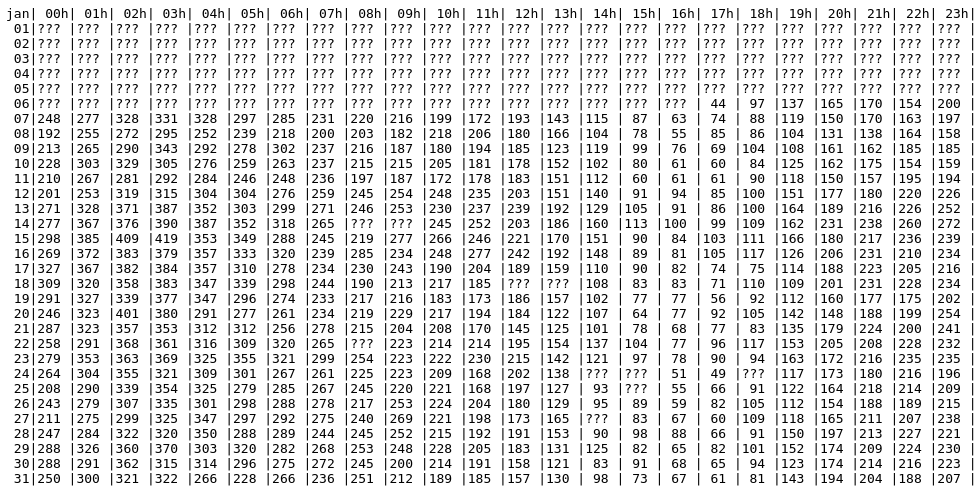
\includegraphics[width=0.9\linewidth]{data/rmob}
		\caption{Text format}
		\label{fig:data:rmob:a}
	\end{subfigure}
	\centering
	\begin{subfigure}{0.475\textwidth}
		\centering
		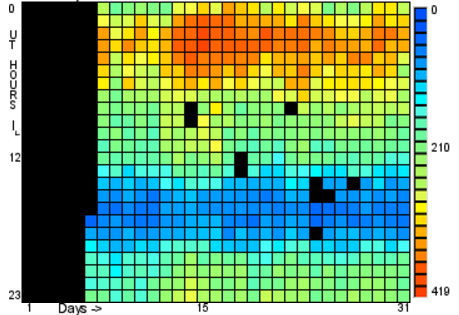
\includegraphics[width=0.9\linewidth]{data/rmob2}
		\caption{Image format}
		\label{fig:data:rmob:b}
	\end{subfigure}
	\caption{RMOB data formats
		\label{fig:data:rmob}}
\end{figure}
The data is collected using the observer's own radio setup. This will include an antenna, and a way of getting the signal to the computer. Typically this is done using a receiver (to control properties of the signal such as squelch) which feeds into the audio port of a computer or laptop. The software works in two parts. \\
The first stage is detecting the meteors from the signal. This is done using HROFFT \cite{hrofft} (figure~\ref{fig:data:hrofft}). 
\begin{figure}[h!]
	\centering
	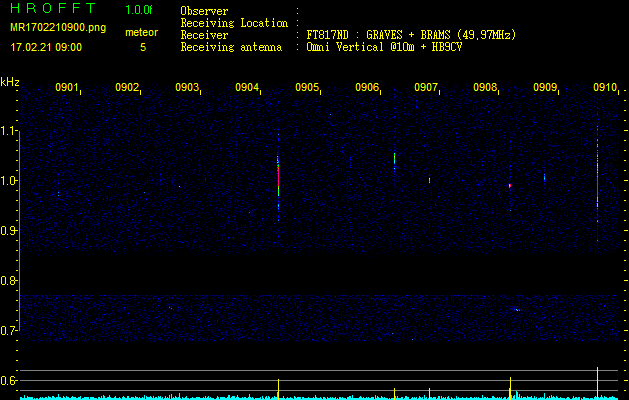
\includegraphics[width=\linewidth]{data/hrofft}
	\caption{HROFFT software screen (courtesy of \cite{hrofftimg})
		\label{fig:data:hrofft}}
\end{figure}\\
As can be seen in figure~\ref{fig:data:hrofft}, the intensity of the signal is calculated and shown in a light blue colour. The full waterfall plot is shown above this, making up the main part of the screen, much the same as figure~\ref{fig:data:rmob:b}. When the intensity of the signal goes over a threshold, it is noted as a meteor (yellow spike). The first threshold is 25dB, the second is 50dB and the third is 75dB. This information is then passed onto Colorgramme Lab. \\
In Colorgramme Lab, the counts are converted to text format and stored as seen in figure~\ref{fig:data:rmob:a}. At the end of the month, this data is uploaded to RMOB.

\section{Data collection \& storage}
\paragraph{Collection\\}
I have collected the data using web scraping. This is a process where a program (mine is written in Python) goes to a webpage, finds all the links on the page, and returns them. By going through each page of data available on the website, I could then download each text file, for each observer, for each month, for each year.\\
\paragraph{Storage\\}
I created two `objects' in Python in order to store the data. Objects are similar to real life objects --- self-contained elements that have their own properties. In the case of the RMOB data, it can be easily split into observers (the stations or people detecting the meteors) and `entries': monthly collections of data (a single text file from RMOB).\\
Using the links collected from web scraping, each file was downloaded, formatted, and loaded into an entry. The data is not stored as part of the entry: the formatted file is saved to a folder. The formatting itself is so that the data is easy to use. Instead of storing the counts using `` $|$ '' to separate the hours, I am using simple commas (``,'') to separate the hours. Instead of using ``???'' to denote unavailable data, I am using ``-1''. This makes it easier both to load the data, and to remove empty data.\\
Each entry has properties: the source of the data (the location in my filesystem that the data is stored), the date (in the format YYYY-MM) and the data itself. Storing every single item of data would be inefficient, so the data must be loaded by calling \texttt{entry.loadData()} first. This opens the location in my filesystem, loads the .csv file, and thus makes the data available for processing. \\
Each of these entries is stored in an `observer' object. This is done by storing the entries in a dictionary, so that the correct data can be selected by specifying the month which is associated with the month of the entry. Some RMOB text files include properties of the detection setup, such as antenna, location, and frequencies. These are stored as part of the observer object as attributes. This allows an easier analysis, since while (for example) assessing spatial variation, the GMAP location can be selected by typing \texttt{observer.locationAttr[`latitudeGMAP']}. Where two entries for the same observer differ, there is a `collision'. In this event, two separate observers are stored.
\section{Final data set}
Figure~\ref{fig:data:contr} shows how many observers contributed to RMOB each month since 2000. Overall, there are 345 observers in my data set, with 5110 entries in total. This means, at most, I have 3,800,000 hourly counts. As can be seen in the figure, more and more observers are uploading each month. This can only mean good things for radio meteor detection analysis!
\begin{figure}[h!]
	\centering
	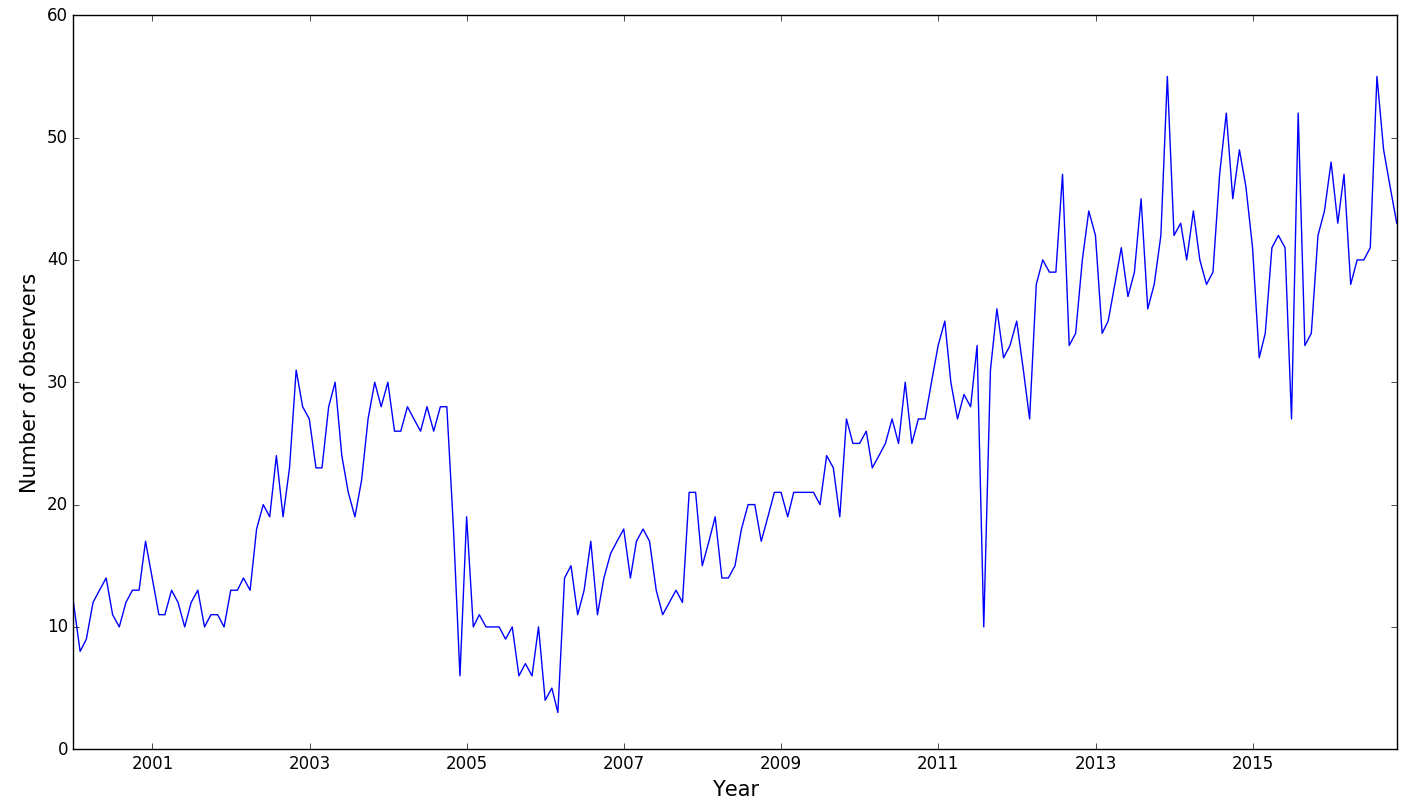
\includegraphics[width=\linewidth]{data/contributing_authors}
	\caption{Number of observers contributing each month
		\label{fig:data:contr}}
\end{figure}\\
Figure~\ref{fig:data:loc} shows the locations represented in the data set. There is clearly a wide variety of locations, across the globe, which will make an analysis of spatial variation valid and worthwhile. 
\begin{figure}[h!]
	\centering
	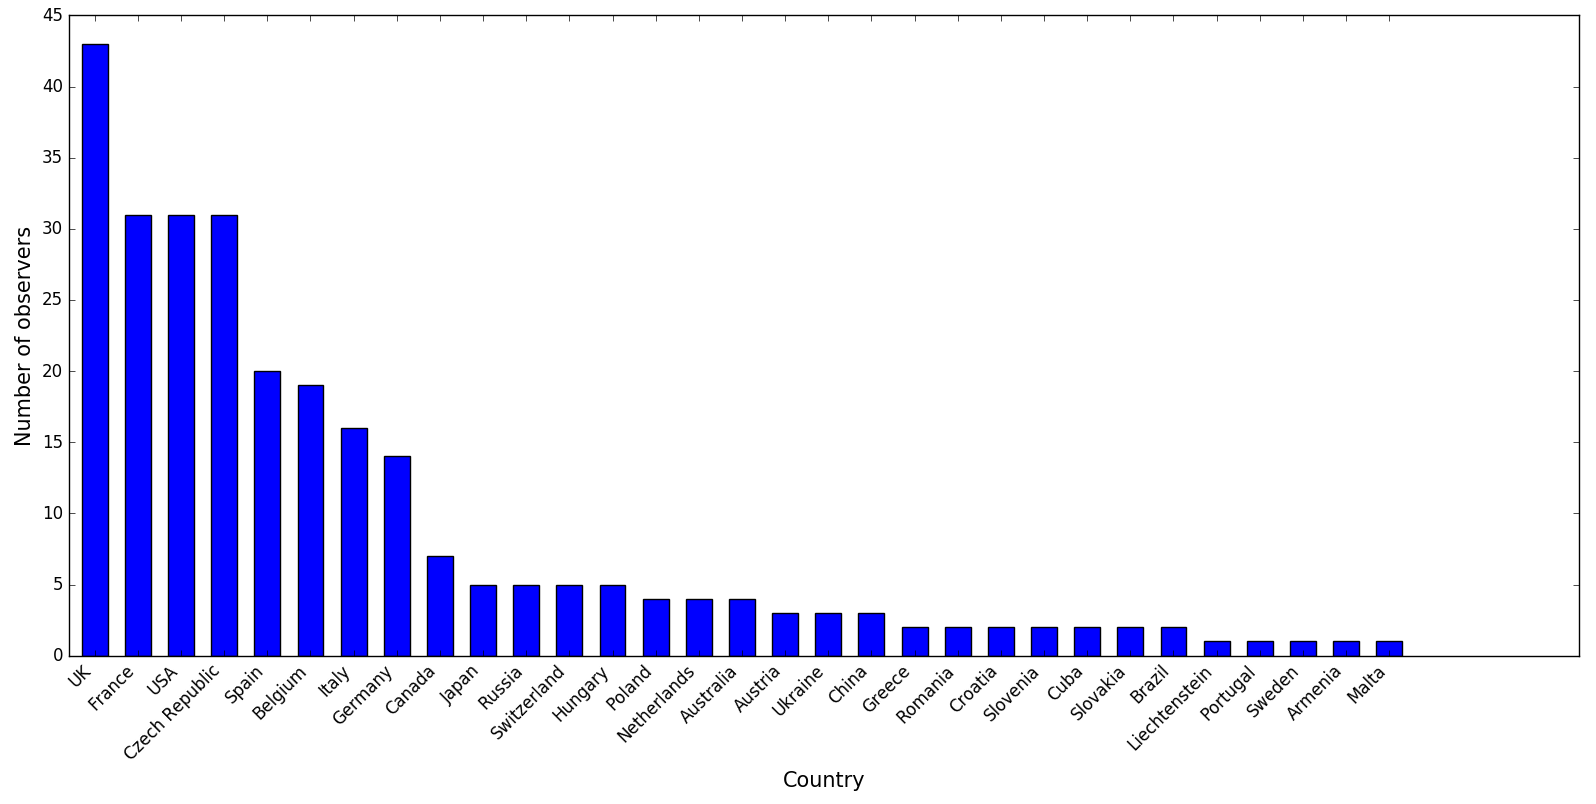
\includegraphics[width=\linewidth]{data/locations}
	\caption{Locations of observers (where known)
		\label{fig:data:loc}}
\end{figure}\\
Figures~\ref{fig:data:locvol} and \ref{fig:data:locavg} show the volume of data available for each country, and the average number of entries uploaded each month.
\begin{figure}[h!]
	\centering
	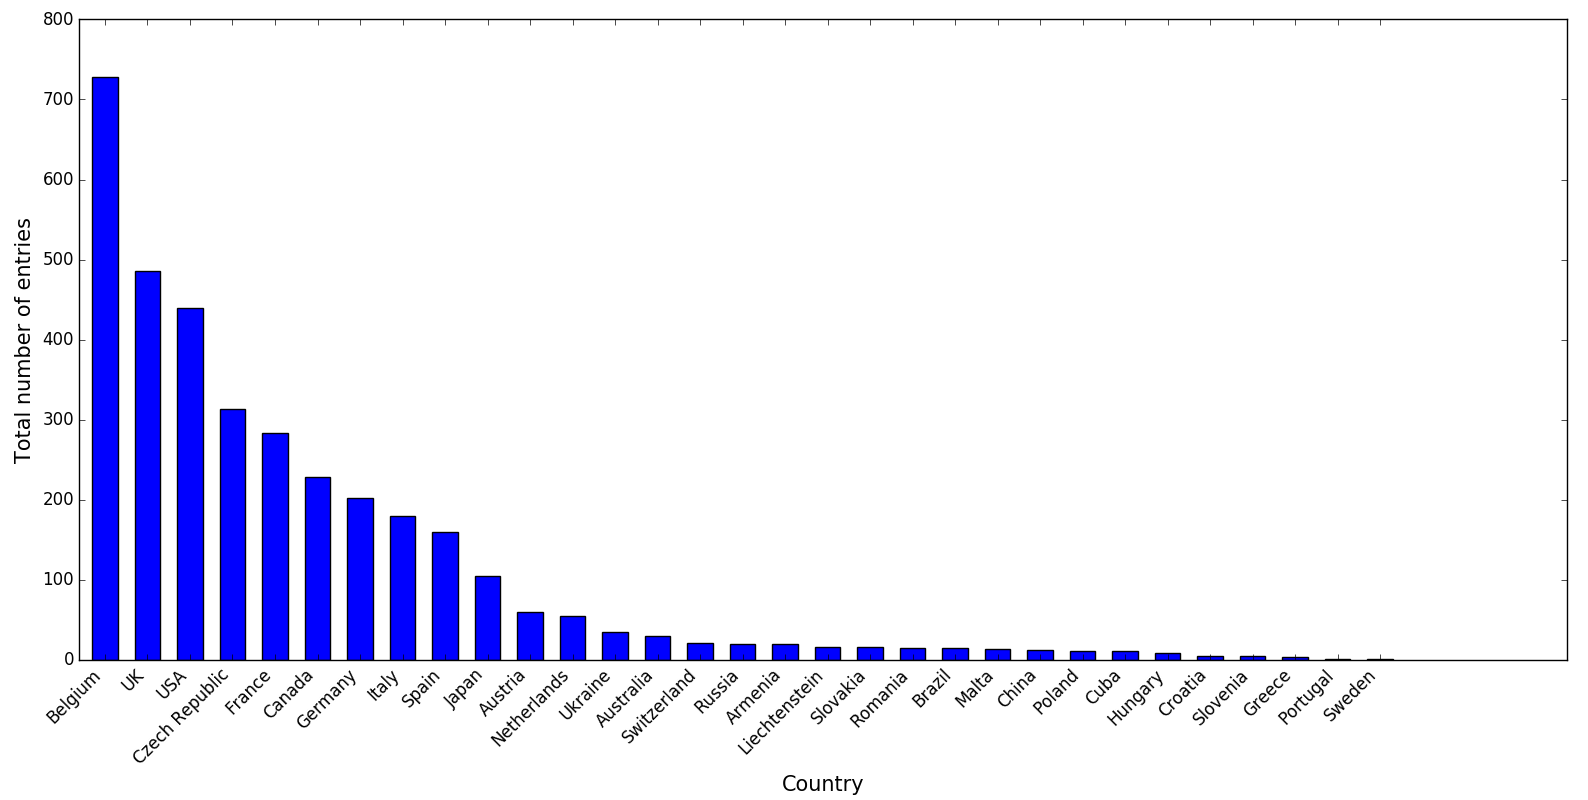
\includegraphics[width=\linewidth]{data/locationsVolume}
	\caption{Volume of data from each location (where known)
		\label{fig:data:locvol}}
\end{figure}
\begin{figure}[h!]
	\centering
	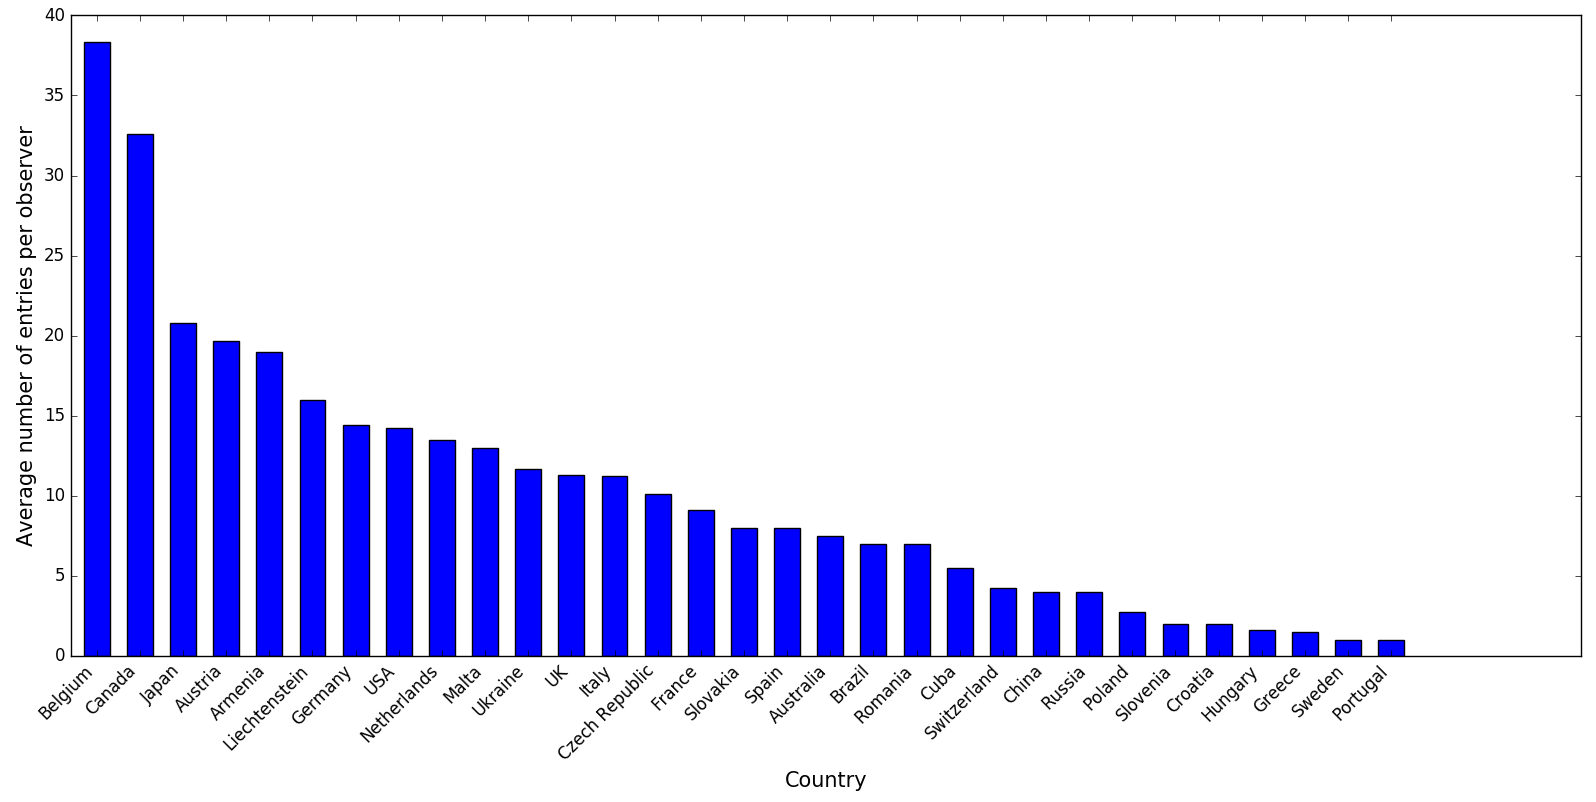
\includegraphics[width=\linewidth]{data/locationsAvg}
	\caption{Average number of entries per month from each location (where known)
		\label{fig:data:locavg}}
\end{figure}